\chapter{Implementation}

\todo{write intro}

% In this chapter, we put forth our research and implementation. First, we
% analyze previous work regarding gas consumption, cost in fiat and security.
% Then we gradually describe our improved methodology that eliminates storage by
% utilizing hash-and-resubmit technique and delivers a gas-efficient, superlight
% Bitcoin client implementation.

\section{Storage vs Memory}

We will first demonstrate the difference in gas usage between storage and
memory for a smart contract in Solidity. Suppose that we have the following
simple contract:

\lstinputlisting[language=Solidity, label={listing:storage_memory},
caption={Solidity test for storage and memory}]{code/StorageVsMemory.sol}

Function \texttt{withStorage()} populates an array saved in storage and
function \texttt{withMemory()} populates an array saved in memory. We
initialize the sizes of the arrays by passing the variable \textsf{size} to the
contract constructor. We run this piece of code for \texttt{size} from 1 to
100. The results are displayed at Figure~\ref{figure:memory_vs_storage}. For
\textsf{size} equal to 100, the gas expended is 53,574 gas units using memory
and 2,569,848 using storage which is almost 50 times more expensive. This code
was compiled with Solidity version 0.6.6 with optimizations
enabled\footnote{This version of Solidity compiler, which was the latest at the
time this paper was published, did not optimize-out any of the variables.}. The
EVM we used  was Ganache at the latest Istanbul\footnote{A summary of Istanbul
fork can be found in the following link:
\url{https://eth.wiki/roadmap/istanbul}} fork. It is obvious that, if there is
the option to use memory instead of storage in the design of smart contracts,
the choice of memory greatly benefits the user.

\begin{figure}
\centering
\begin{tikzpicture}
    \begin{axis}[
        y tick label style={/pgf/number format/.cd,%
          set thousands separator={,},
          fixed},
        legend pos=north west,
        scaled y ticks = false,
        grid=major,
        xlabel={Array size},
        ylabel={Gas consumption}]
    \addplot table [mark=none, col sep=comma] {data/storage.csv};
    \addplot table [mark=none, col sep=comma] {data/memory.csv};
    \legend{$storage$,$memory$};
\end{axis}
\end{tikzpicture}
\caption{Gas consumption for memory and storage}
\label{figure:memory_vs_storage}
\end{figure}


\section{The Hash-and-Resubmit Pattern}

We now introduce a novel design pattern for Solidity smart contracts that
results into significant gas optimization due to the elimination of expensive
storage operations. We first introduce our pattern, and display how smart
contracts benefit from using it. Then, we proceed into integrating our pattern
in the NIPoPoW protocol, and we analyze the performance in comparison with
previous work~\cite{gglou}.

\subsection{Motivation}
It is essential for smart contracts to store data in the blockchain. However,
interacting with the storage of a contract is among the most expensive
operations of the EVM~\cite{wood, buterin}. Therefore, only necessary data
should be stored and redundancy should be avoided when possible. This is
contrary to conventional software architecture, where storage is considered
cheap. Usually, the performance of data access in traditional systems is
related with time. In Ethereum, however, performance is related to gas
consumption. Access to persistent data costs a substantial amount of gas, which
has a direct monetary value.

One way to mitigate gas cost of reading variables
from the blockchain is to declare them as public. This leads to the creation of a
\emph{getter} function in the background, allowing free access to the value of
the variable. But this treatment does not prevent the initial population of
storage data and write operations which are significantly expensive for large
sizes of data.

By using the \emph{hash-and-resubmit} pattern, large structures are omitted
from storage entirely, and are contained in memory. When a function call is
performed, the signature and arguments of the function are included in the
transactions field of the body of a block. The contents of blocks are public to
the network, therefore this information is locally available to full nodes. By
simply observing blocks, a node retrieves data sent to the contract by other
users. To interact publicly with this data without the utilization storage, the
node \emph{resends} the observed data to the blockchain. The concept of
resending data is redundant in conventional systems. However, this technique
is very efficient to use in Solidity due to the significantly lower gas cost
of memory operations in relation with storage operations.

\subsection{Related patterns} Towards implementing gas-efficient smart
contracts~\cite{contract-opt-1, contract-opt-2, slither, madmax}, several
methodologies have been proposed. In order to eliminate storage operations
using data signatures, the utilization of IPFS~\cite{ipfs} is proposed by
\cite{ipfs-1} and~\cite{ipfs-2}. However, these solutions do not address
availability, which is one of our main requirements. Furthermore,
\cite{logs} uses logs to replace storage in a similar manner, sparing a great
amount of gas. However, this approach does not address consistency, which is
also one of our critical targets. Lastly, ~\cite{memory-array} proposes an
efficient manner to replace read storage operations, but does not address write
operations.

\subsection{Applicability}
We now list the requirements an application needs to meet in order to benefit
from the \emph{hash-and-resubmit} pattern:

\begin{enumerate}
    \item The application is a Solidity smart contract.
    \item Read/write operations are performed in large arrays that exist in
        storage. Using the pattern for variables of small size may result in
        negligible gain or even performance loss.
    \item A full node observes function calls to the smart contract.
\end{enumerate}

\subsection{Participants and collaborators} The first participant is the
smart contract $\contract$ that accepts function calls. Another participant is
the invoker $\invoker$, who dispatches a large array $\data_0$ to $\contract$
via a function \texttt{\proc$_1$}($\data_0$). Note that $\data_0$ is
potentially processed in $\proc_1$, resulting to $\data$. The last participant
is the observer $\observer$, who is a full node that observes transactions
towards $\contract$ in the blockchain. This is possible because nodes maintain
the blockchain locally. After observation, $\observer$ retrieves data $\data$.
Since this is an off-chain operation, a malicious $\observer$ potentially
alters $\data$ before interacting with $\contract$. We denote the
potentially modified $\data$ as $\datas$. Finally, $\observer$ acts as an
invoker by making a new call to $\contract$, \texttt{\proc$_2$}($\datas$). The
verification that $\data = \datas$, which is a prerequisite for the secure
functionality of the underlying contract, consists a part of the pattern and is
performed in \texttt{\proc$_2$}.

\subsection{Implementation} The implementation of this pattern is
divided in two parts. The first part covers how $\datas$ is retrieved by
$\observer$, whereas in the second part the verification of $\data=\datas$ is
realized. The challenge here is twofold:

\begin{enumerate}

    \item Availability: $\observer$ must be able to retrieve $\data$ without
        the need of accessing on-chain data.

    \item Consistency: $\observer$ must be prevented from dispatching $\datas$
        that differs from $\data$ which is a product of originally submitted
        $\data_0$.

\end{enumerate}

\emph{Hash-and-resubmit} technique is performed in two
stages to face these challenges: (a) the \emph{hash} phase, which addresses
\emph{consistency}, and (b) the \emph{resubmit} phase which addresses
\emph{availability} and \emph{consistency}.

\subsubsection{Addressing Availability} During the \emph{hash} phase,
$\invoker$ makes the function call \texttt{\proc}$_1$($\data_0$). This
transaction, which includes a function signature (\texttt{\proc$_1$}) and the
corresponding data ($\data_0$), is added in a block by a miner. Due to
blockchain's transparency, the observer of \texttt{\proc}$_1$, $\observer$,
retrieves a copy of $\data_0$ from the calldata, without the need of accessing contract data. In
turn, $\observer$ performs \emph{locally} the same set of on-chain instructions
operated on $\data_0$, generating $\data$. Thus, availability is addressed
through observability.

\subsubsection{Addressing Consistency} We prevent an adversary $\observer$
from dispatching data $\datas\neq\data$ by storing the \emph{signature} of
$\data$ in the contract's state during the execution of \texttt{\proc$_1$(.)} by
$\invoker$. In the context of Solidity, a signature of a structure is the
digest of the structure's \emph{hash}. The pre-compiled \texttt{sha256} is
convenient to use in Solidity, however we can make use of any cryptographic
hash function \textsf{H()}: \[\textsf{hash} \gets \textsf{H}(\textsf{d})\]
Then, in \emph{rehash} phase, the verification is performed by comparing the
stored digest of $\data$ with the digest of $\datas$:
\[\textsf{require}(\textsf{hash} = \texttt{H}(\datas))\] \noindent In Solidity,
the size of this digest is 32 bytes. To persist such a small value in the
contract's memory only adds a constant, negligible cost overhead. We illustrate
the application of the \emph{hash-and-resubmit} pattern in
Figure~\ref{fig:har-pattern}.

\begin{figure*}[h]
    \begin{center} 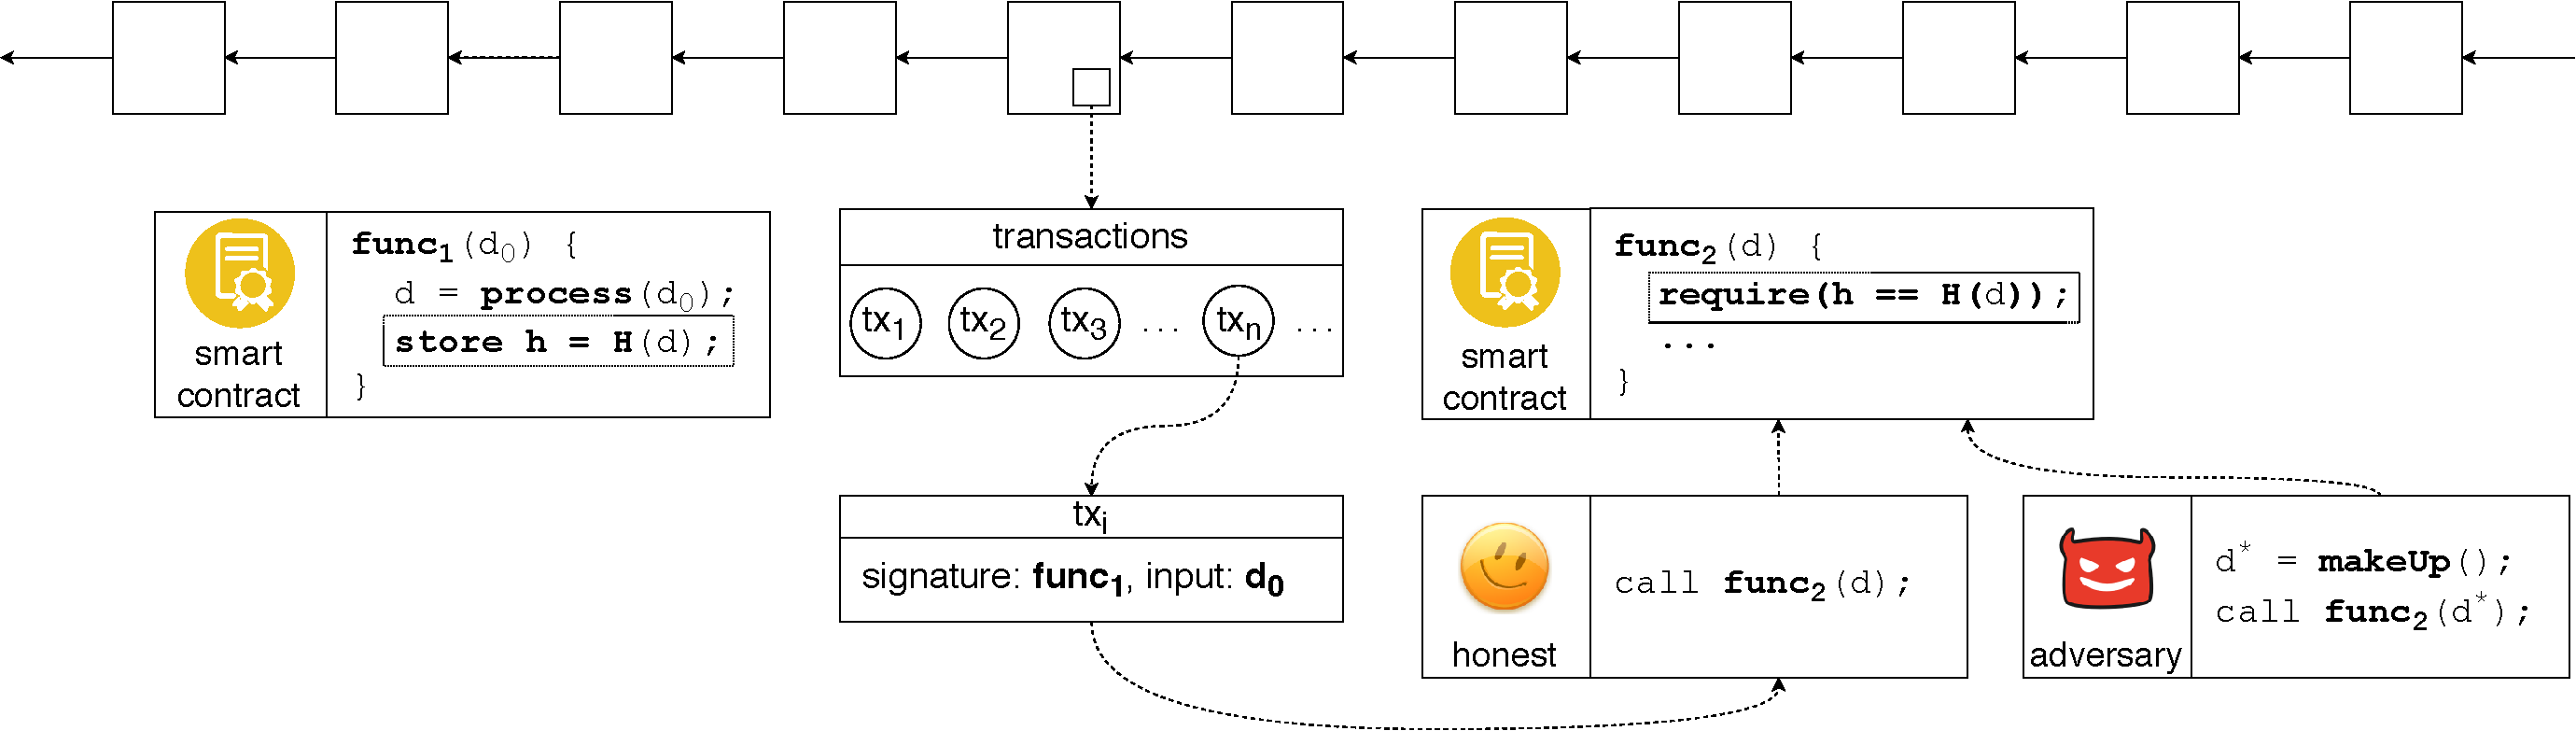
\includegraphics[width=0.8\textwidth]{figures/har-pattern.pdf}
    \end{center}

    \caption{The \emph{hash-and-resubmit} pattern. First, an invoker calls
        \proc$_1$($\data_0$). $\data_0$ is processed \emph{on-chain} and
        $\data$ is generated. The signature of $\data$ is stored in the
        blockchain as the digest of a hash function \textsf{H}(.). Then,
        a full node that observes invocations of $\proc_1$ retrieves $\data_0$,
        and generates $\data$ by performing the analogous processing on
        $\data_0$ \emph{off-chain}. An adversarial observer dispatches
        $\datas$, where $\datas$$\neq$$\data$. Finally, the nodes invoke
        $\proc_2$(.). In $\proc_2$, the validation of input data is performed,
        reverting the function call if the signatures of the input does not
        match with the signature of the originally processed data. By applying
        a \emph{hash-and-resubmit pattern}, only the fixed-size signature of
        $\data$ is stored to the contract's state, replacing arbitrarily large
        structures.}

        \label{fig:har-pattern}
\end{figure*}


\subsection{Sample} We now demonstrate the usage of the
hash-and-resubmit pattern with a simplistic example. We create a smart contract
that orchestrates a game between two players, $\pla$ and $\plb$. The winner is
the player with the most valuable array. The interaction between players
through the smart contract is realized in two phases: (a) the submit phase and
(b) the contest phase.

\noindent\textbf{Submit phase:} $\pla$ submits an N-sized array, $\arra$, and
becomes the $\holder$ of the contract.

\noindent\textbf{Contest phase:} $\plb$ submits $\arrb$. If the result of
\textsf{compare}($\arrb$, $\arra$) is \true, then $\plb$ becomes the holder.

% \begin{algorithm}
    \caption{\label{alg:game-storage}\textsf{best array} using storage}
    \begin{algorithmic}[1]

    \Contract{best-array}
        \State{$\textsf{best} \gets \emptyset$;
               $\textsf{holder} \gets \emptyset$}
        \Function{\sf submit}{$a$}
        \State \textsf{best} $\gets a$
            \Comment{array saved in storage}
            \State \textsf{holder $\gets$ msg.sender}
        \EndFunction

        \Function{\sf contest}{$a$}
            \State \textsf{require}(\textsf{compare}($a$))
            \State \textsf{holder} $\gets$ \textsf{msg.sender}
        \EndFunction

        \Function{\sf compare}{$a$}
            \State \textsf{require}($|a|$ $\geq$ $|$\textsf{best}$|$)
            \For{$i$ \textbf{in} $|$\textsf{best}$|$}
            \State \textsf{require}($a[i]$ $\geq$ \textsf{best}[i])
            \EndFor
            \State \Return{true}
        \EndFunction
        \EndContract
        \vskip8pt
    \end{algorithmic}
\end{algorithm}

\begin{algorithm}
    \caption{\label{alg:game-memory}\textsf{best array} using hash-and-resubmit pattern}
    \begin{algorithmic}[1]
        \Contract{best-array}
        \State{$\textsf{hash} \gets \emptyset$;
               $\textsf{holder} \gets \emptyset$}

        \Function{\sf submit}{$\arra$}
        \State $\textsf{hash} \gets \textsf{H}(\arra)$
            \Comment{hash saved in storage}
            \State \textsf{holder} $\gets$ \textsf{msg.sender}
        \EndFunction

    \Function{\sf contest}{$\arra^*$, $\arrb$}
    \State \textsf{require}(\textsf{hash256}($\arra^*$) $=$ $hash$)
        \Comment{validate $\arra^*$}
        \State \textsf{require}(\textsf{compare}($\arra^*$, $\arrb$))
        \State \textsf{holder} $\gets$ \textsf{msg.sender}
    \EndFunction
    \Function{\sf compare}{$\arra^*$, $\arrb$}
        \State \textsf{require}($|\arra^*|$ $\geq$ $|\arrb|$)
        \For{$i$ \textbf{in} $|\arra^*|$}
            \State \textsf{require}($\arra^*[i] \geq \arrb[i]$)
        \EndFor
    \EndFunction
    \State \Return{true}
    \EndContract
    \vskip8pt
    \end{algorithmic}
\end{algorithm}


We provide a simple implementation for \textsf{compare}, but we can consider
any notion of comparison, since the pattern is abstracted from such
implementation details.

We make use of the \emph{hash-and-resubmit} pattern by prompting $\plb$ to
provide \emph{two} arrays to the contract during contest phase: (a) $\arras$,
which is the originally submitted array by $\pla$, possibly modified by $\plb$,
and (b) $\arrb$, which is the contesting array.

We provide two implementations of the above described game.  In
Listing~\ref{listing:har-sample} we display the storage implementation (left),
and the memory implementation (right) embedding the \emph{hash-and-resubmit}
pattern.

\lstinputlisting[language=Solidity, label={listing:har-sample},
caption={Implementation of sample.}]{code/HarGame.sol}

\subsection{Gas analysis} The gas consumption of the two above
implementations is displayed in Figure~\ref{fig:har-example}. By using the
\emph{hash-and-resubmit} pattern, the aggregated gas consumption for
\textsf{submit} and \textsf{contest} is decreased by 95\%. This significantly
affects the efficiency and applicability of the contract. Note that the storage
implementation exceeds the Ethereum block gas limit ($10{,}000{,}000$ gas as of
June 2020), for arrays of size 500 and above, contrary to the optimized
version, which consumes approximately only $1/10^{th}$ of the block gas limit
for arrays of $1{,}000$ elements.

\begin{figure}[!h]
\begin{center}
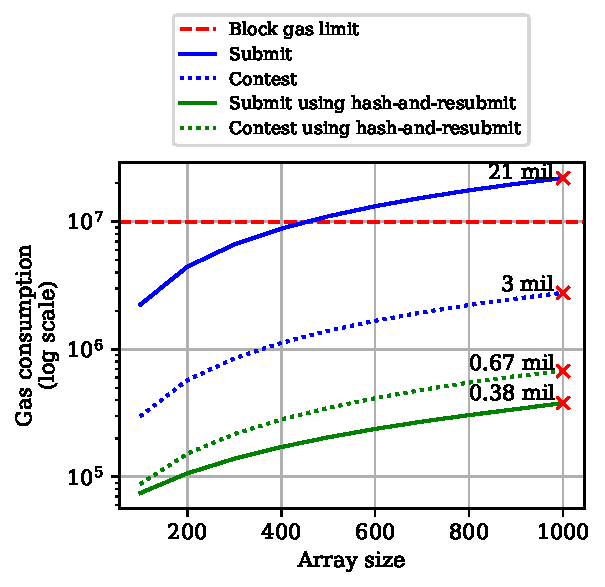
\includegraphics[width=0.6 \columnwidth]{figures/har-example.pdf}
\end{center}
\caption{Gas-cost reduction using the \emph{hash-and-resubmit} pattern (lower
is better). By avoiding gas-heavy storage operations, the aggregated cost of
\textsf{submit} and \textsf{contest} is decreased by 95\%.}
\label{fig:har-example}
\end{figure}

\subsection{Consequences} The most obvious consequence of applying the
\emph{hash-and-resubmit} pattern is the circumvention of storage
structures, a benefit that saves a substantial amount of gas, especially when
these structures are large. To that extent, smart contracts that exceed the
Ethereum block gas limit and benefit sufficiently for the alleviation of
storage structures are becoming practical. Furthermore, the pattern enables
off-chain transactions, significantly improving the performance of smart
contracts.

\subsection{Known Uses} To our knowledge, we are the first to address
consistency and availability by combining blockchain's transparency with data
structures signatures in a manner that eliminates storage variables from
smart contracts.

\subsection{Enabling NIPoPoWs} We now present how the
\emph{hash-and-resubmit} pattern is used in the context of the NIPoPoW
superlight client. The NIPoPoW verifier adheres to a submit-and-contest schema
where the inputs of the functions are arrays that are processed on-chain, and a
node observes function calls towards the smart contract.  Therefore, it
makes a suitable case for our pattern.

In the \emph{submit} phase, a \emph{proof} is submitted. In the case of falsity, it
is contested by another user in \emph{contest} phase. The contester is a node
that monitors the traffic of the verifier. The input of \textsf{submit}
function includes the submit proof ($\pis$) that indicates the occurrence of an
\emph{event} ($e$) in the source chain, and the input of \textsf{contest}
function includes a contesting proof ($\pic$). A successful contest of $\pis$
is realized when $\pic$ has a better score~\cite{nipopows}. In this section, we
will not examine the score evaluation process since it is irrelevant to the
pattern. The size of proofs is dictated by the value $m$. We consider $m$ = 15
to be sufficiently secure~\cite{nipopows}.

In previous work, NIPoPoW proofs are maintained on-chain, resulting in
extensive storage operations that limit the applicability of the verifier
considerably. In our implementation, proofs are not stored on-chain, and $\pis$
is retrieved by the contester from the calldata. Since we
assume a trustless network, $\pis$ is altered by an adversarial contester. We denote
the potentially changed $\pis$ as $\pisa$. In \emph{contest} phase, $\pisa$ and
$\pic$ are dispatched in order to enable the \emph{hash-and-resubmit} pattern.

For our analysis, we create a blockchain similar to the Bitcoin chain with the
addition of the interlink structure in each block as in~\cite{gglou}. Our chain
spans 650,000 blocks, representing a slightly enhanced Bitcoin
chain\footnote{Bitcoin spans $633{,}022$ blocks as of June 2020. Metrics by
\url{https://blockchain.com/}}. From the tip of our chain, we branch two
sub-chains that span 100 and 200 additional blocks respectively, as illustrated
in Figure~\ref{fig:chains}. Then, we use the smaller chain to create $\pis$,
and the larger chain to create $\pic$. We apply the protocol by submitting
$\pis$, and contesting with $\pic$. The contest is successful, since $\pic$
represents a chain consisting of greater number of blocks than $\pis$,
therefore encapsulating more proof-of-work. We select this setting as it
provides maximum code coverage, and it describes the most gas-heavy scenario
for the verifier.

In Algorithm~\ref{alg:har-nipopow} we show how \emph{hash-and-resubmit} pattern
is embedded into the NIPoPoW client.

\begin{figure}[!h]
    \begin{center}
        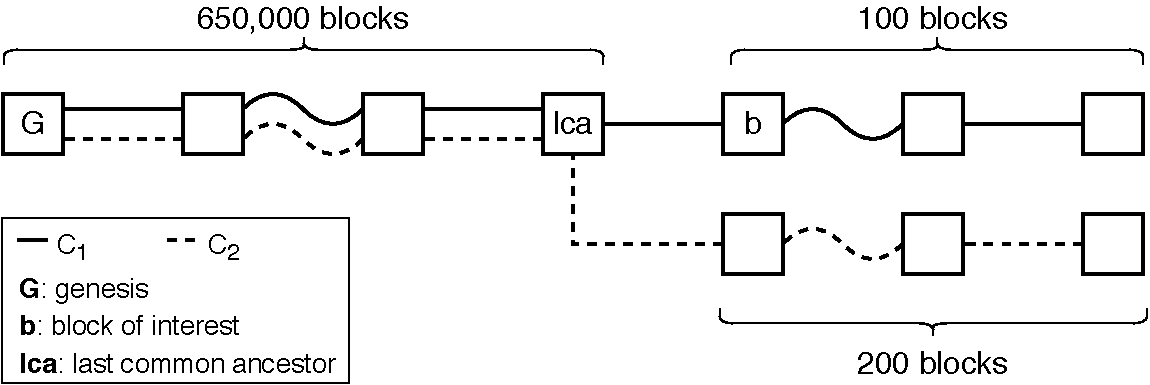
\includegraphics[width=0.6\columnwidth]{figures/nipopow-subm-cont}
    \end{center}
    \caption{Forked chains for our gas analysis.}
    \label{fig:chains}
\end{figure}

In Figure~\ref{fig:har-nipopow}, we display how the \emph{hash-and-resubmit}
provides an improved implementation compared to previous work. The graph
illustrates the aggregated cost of \emph{submit} and \emph{contest} phases for
each implementation. We observe that, by using the \emph{hash-and-resubmit}
pattern, we achieve to increase the performance of the contract by 50\%. This
is a decisive step towards creating a practical superlight client.

Note that gas consumption generally follows an ascending trend, however it
is not a monotonically increasing function. This is due to the fact that
NIPoPoWs are probabilistic structures, the size of which is determined by the
distribution of superblocks within the underlying chain. A proof that is
constructed for a chain of a certain size can be larger than a proof
constructed for a slightly smaller chain, resulting in non-monotonic increase
of gas consumption between consecutive values of proof sizes.

\newcommand{\genesis}{\textsf{G}}

\begin{algorithm}
    \label{alg:har-nipopow}
    \caption{The \textsf{NIPoPoW} client using hash-and-resubmit pattern}
    \begin{algorithmic}[1]

    \Contract{crosschain}
    \State $\textsf{events} \gets \bot;$ $\genesis \gets \bot$
    \Function{\sf initialize}{$\genesis_{remote}$}
        \State \genesis $\gets \genesis_{remote}$
    \EndFunction
    \Function{\sf submit}{$\pis$, $e$}
        \State \textsf{require}($\pis$[0] = $\genesis$)
        \State \textsf{require}($\textsf{events$[e]$} = \bot$)
        \State \textsf{require}($\textsf{valid-interlink}(\pi)$)
        \State \textsf{DAG} $\gets$ \textsf{DAG} $\cup$ $\pis$
        \State \textsf{events$[e]$.hash} $\gets$ \textsf{H}($\pis$)
        \Comment{enable pattern}
        \State \textsf{ancestors} $\gets$ \textsf{find-ancestors()}
        \State \textsf{events$[e]$.pred} $\gets$
            \textsf{evaluate-predicate}(\textsf{ancestors}, e)
        \State \textsf{ancestors} $=$ $\bot$
    \EndFunction
    \Function{\sf contest}{$\pisa$, $\pic$, $e$}
        \Comment{provide proofs}
        \State \textsf{require}(\textsf{events$[e]$.hash} $=$ \textsf{H}($\pisa$))
        \Comment{verify $\pisa$}
        \State \textsf{require}($\pic$[0] = $\genesis$)
        \State \textsf{require}(\textsf{events}$[e]$ $\ne$ $\bot$)
        \State \textsf{require}(\textsf{valid-interlink}($\pi_{cont}$))
        \State $lca$ = \textsf{find-lca}($\pisa$, $\pic$)
        \State \textsf{require}(\textsf{score}($\pic[:lca]$)
            $>$ \textsf{score}($\pisa[:lca]$))
        \State \textsf{DAG} $\gets$ \textsf{DAG} $\cup$ $\pic$
        \State \textsf{ancestors} $\gets$ \textsf{find-ancestors}(\textsf{DAG})
        \State \textsf{events$[e]$.pred} $\gets$
            \textsf{evaluate-predicate}(\textsf{ancestors}, $e$)
        \State \textsf{ancestors} $=$ $\bot$
    \EndFunction
    \EndContract
    \vskip8pt
    \end{algorithmic}
\end{algorithm}



\begin{figure}[H]
    \begin{center}
        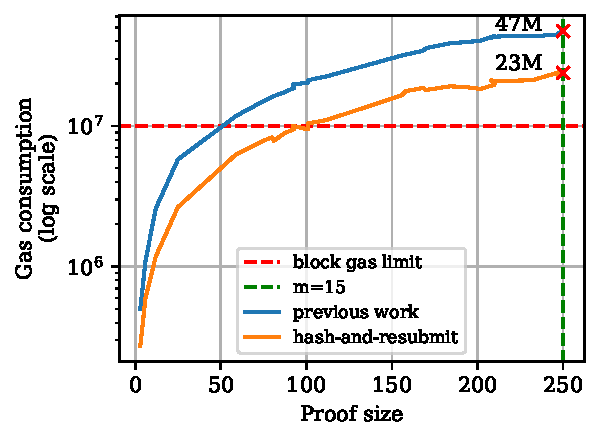
\includegraphics[width=0.6\columnwidth]{figures/har-nipopows.pdf}
    \end{center}
    \caption{Performance improvement using hash-and-resubmit pattern in
        NIPoPoWs compared to previous work for a secure value of $m$ (lower is
        better). The gas consumption is decreased by approximately 50\%.}
    \label{fig:har-nipopow}
\end{figure}

\section{Hash-and-Resubmit Variations}
In order to enable selective dispatch of a segment of interest, different
hashing schemas can be adopted, such as Merkle Trees ~\cite{merkle} and Merkle Mountain
Ranges ~\cite{mmr-1, mmr-2}. In this variation of the pattern, which we term
\emph{merkle-hash-and-resubmit}, the signature of an array $\data$ is
Merkle Tree Root (MTR). In the \emph{resubmit} phase, $\data[m{:}n]$ is
dispatched, accompanied by the siblings that reconstruct the MTR of
$\data$.

\begin{figure}[h]
    \begin{center}
        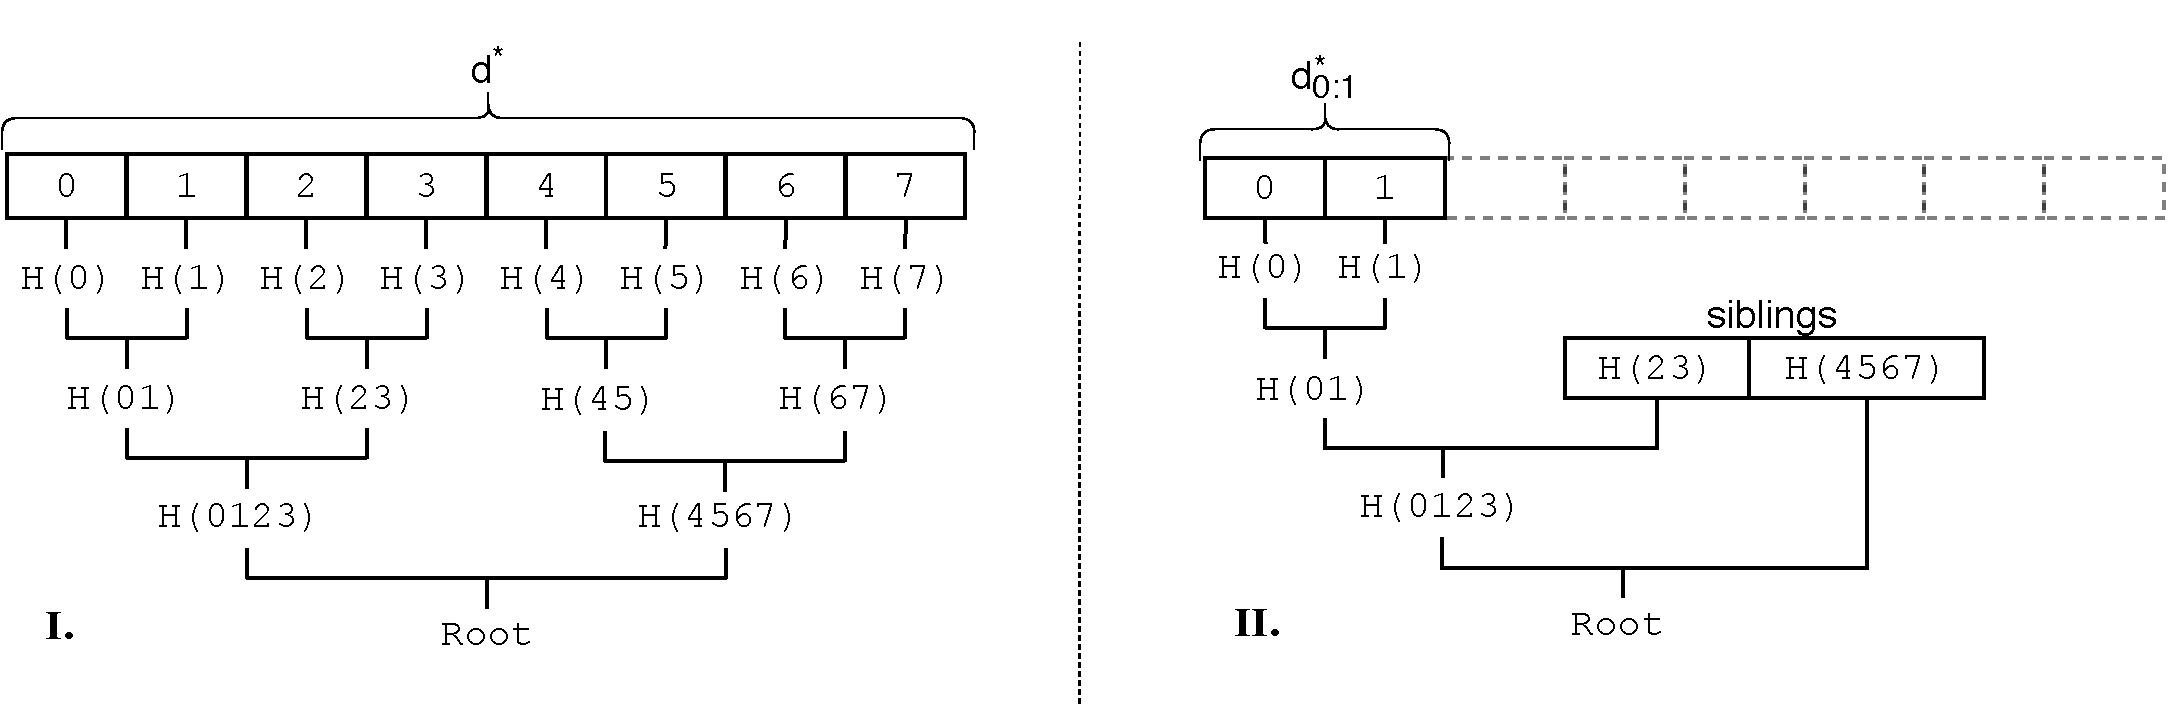
\includegraphics[width=1\linewidth]{figures/merkle-har.pdf}
    \end{center}
    \caption{\textbf{I.} The calculation of root in \emph{hash} phase.
    \textbf{II.} The verification of the root in \emph{resubmit} phase.
    \textsf{H}($k$) denotes the digest of element $k$. \textsf{H}($kl$) denotes the
    result of \textsf{H}(\textsf{H}($k$) $|$ \textsf{H}($l$))}
    \label{fig:merkle-har}
\end{figure}

This variation of the pattern removes the burden of sending redundant data,
however it implies on-chain construction and validation of the Merkle
construction. In order to construct a MTR for an array $\data$,
$|\data|$ hashes are needed for the leafs of the MT, and $|\data| -
1$ hashes are needed for the intermediate nodes. For the verification, the
segment of interest $\data[m{:}n]$ and the siblings of the MT are hashed.
The size of siblings is approximately $log_2(|\data|)$. The process of
constructing and verifying the MTR is displayed in Figure
~\ref{fig:merkle-har}.

In Solidity, different hashing operations vary in cost. An invocation of
\textsf{sha256}($\data$), copies $\data$ in memory, and then the
\emph{CALL} instruction is performed by the EVM that calls a pre-compiled
contract. At the current state of the EVM, \emph{CALL} costs 700 gas units, and
the gas paid for every word when expanding memory is 3 gas units~\cite{wood}.
Consequently, the expression $1 \times \textsf{sha256}(\data)$ costs less than
$|\data| \times $\textsf{sha256}(1) operations. A different cost policy applies
for \textsf{keccak}~\cite{keccak} hash function, where hashing costs 30 gas
units plus 6 additional gas far each word for input data~\cite{wood}. The usage
of \textsf{keccak} dramatically increases the performance in comparison with
\textsf{sha256}, and performs better than plain rehashing if the product of
on-chain processing is sufficiently larger than the originally dispatched data.
Costs of all related operations are listed in Table~\ref{tab:operations-gas}.

\begin{table}[!h]
\begin{tabular}{|c|c|}
\hline
\textbf{Operation} & \textbf{Gas cost} \\ \hline
\textsf{load}($\data$)            & $ \data_{bytes} \times 68 $          \\ \hline
\textsf{sha256}($\data$)          & $\data_{words} \times 3 + 700 $     \\ \hline
\textsf{keccak}($\data$)          & $\data_{words} \times 6 + 30 $      \\ \hline
\end{tabular}
\caption{Gas cost of EVM operations as of June 2020.}
\label{tab:operations-gas}
\vspace*{-5mm}
\end{table}


The merkle variation can be potentially improved by dividing $\data$ in
chunks larger than 1 element. We leave this analysis for future work.

\begin{figure}[H]
    \begin{center}
        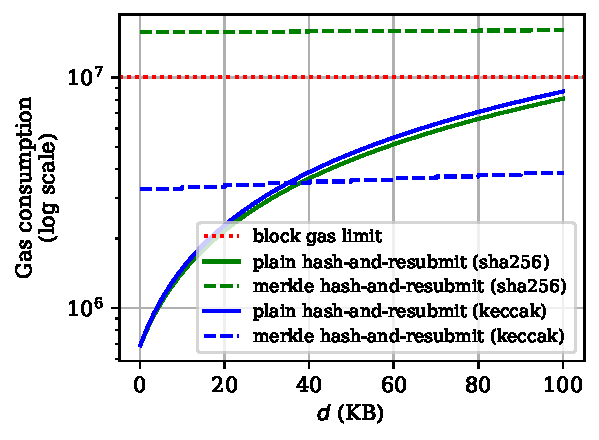
\includegraphics[width=0.5\columnwidth]{figures/har-vs-mhar.pdf}
    \end{center}
    \caption{Trade-offs between \emph{hash-and-resubmit} variations. In the
    vertical axis the gas consumption is displayed. In the horizontal axis the
    size of $\data$. The size of $d_0$ is 10KB bytes, and the hash functions we
    use are the pre-compiled \texttt{sha256} and \texttt{keccak}.}
    \label{fig:har-vs-mhar}
\end{figure}


In Table~\ref{tab:har-vs-mhar} we display the operations needed for hashing and
verifying the underlying data for both variations of the pattern as a function
of data size. In Figure~\ref{fig:har-vs-mhar} we demonstrate the gas
consumption for dispatched data of 10KB, and varying size of on-chain
process product.

\newcommand{\mydata}{\data}

\begin{table}[h]
\begin{tabular}{|c|c|c|}
\hline
\textbf{\begin{tabular}[c]{@{}c@{}}phase per\\variance\end{tabular}} &
\textbf{\begin{tabular}[c]{@{}c@{}}plain hash\\and resubmit\end{tabular}} &
\textbf{\begin{tabular}[c]{@{}c@{}}merkle hash\\ and resubmit\end{tabular}} \\ \hline
\textbf{hash} &
\textsf{H}($\mydata$) &
\begin{tabular}[c]{@{}c@{}}
    \textsf{H}($\mydata_{elem}$) $\times\ |\mydata|$ \\ \textsf{H}(digest)
$\times\ (|\mydata|-1)$

\end{tabular} \\ \hline
\textbf{resubmit} &
\textsf{load}($\mydata$) + \textsf{H}($\mydata$) &
\begin{tabular}[c]{@{}c@{}}
    \textsf{load}($\mydata[m{:}n])$ + \\
    \textsf{load}($siblings$) + \\
    \textsf{H}($\mydata[m{:}n])$ + \\
    \textsf{H}($digest$)$\times |siblings|$
\end{tabular} \\ \hline
\end{tabular}

\caption{Summary of operations for \emph{hash-and-resubmit} pattern variations.
$\mydata$ is the product of on-chain operations and $\mydata_{elem}$ is an
element of $\mydata$. \textsf{H} is a hash function, such as \textsf{sha256}
or \textsf{keccak}, $digest$ is the product of \textsf{H}(.) and $siblings$ are
the siblings of the Merkle Tree constructed for $\mydata$.
}

\label{tab:har-vs-mhar}
\vspace*{-10mm}
\end{table}


\section{Removing Look-up Structures}

Now that we freely eliminate large arrays, we can focus on other
types of storage variables. The challenge we face is that the protocol of
NIPoPoWs depends on a Directed Acyclic Graph (DAG) of blocks which is a
mutable hashmap. This DAG is needed because interlinks of superblocks can be
adversarially defined. By using DAG, the set of ancestor blocks of a block is
extracted by performing a simple graph search. For the evaluation of the
predicate, the set of \emph{ancestors} of the best blockchain tip is used.
Ancestors are created to avoid an adversary who presents an honest chain but
skips the blocks of interest.

This logic is intuitive and efficient to implement in most traditional
programming languages such as C++, JAVA, Python, JavaScript, etc. However, as
our analysis demonstrates, such an implementation in Solidity is significantly
expensive. Albeit Solidity supports constant-time look-up structures, hashmaps
are only contained in storage. This affects the performance of the client,
especially for large proofs.

We make a keen observation regarding potential positions of the \emph{block of
interest} in proofs, which leads us to the construction of an architecture that
does not require a DAG, the ancestors or other complementary structures. To
support this claim, we adopt the notation from~\cite{nipopows}. We also
consider the predicate $\pred$ to be of the type: ``does block $\boi$ exist
inside proof $\pr$?'', where $\boi$ denotes the block of interest of proof
$\pr$. The entity that performs the submission is $\es$, and the entity that
initiates a contest is $\ec$.

\subsection{Position of Block of Interest} NIPoPoWs are sets of sampled
interlinked blocks, meaning that they can be perceived as chains. Since proofs
$\pis$ and $\pic$ differ, a fork is created at the index of
their last common ancestor ($\lca$). The block of interest lies at a certain
index within $\pis$ and indicates a stable predicate~\cite{nipopows,
generic-client} that is $\true$ for $\pis$. A submission in which $\boi$ is
absent from $\pis$ is aimless, because it automatically fails since no element
of $\pis$ satisfies $\pred$. On the contrary, $\pic$ tries to prove the
\emph{falseness} of the underlying predicate. This means that, if the block of
interest is included in $\pic$, then the contest is aimless. We freely use the
term aimless to also characterize components that are included in such actions
i.e.\ aimless proof, aimless blocks etc. We use the term meaningful to describe
non-aimless actions and components.

\newcommand{\block}{\mathsf{B}}

In the NIPoPoW protocol, proofs' segments $\pis\{{{:}}\lca\}$ and
$\pic\{{:}\lca\}$ are merged to prevent adversaries from skipping
blocks, and the predicate is evaluated against $\pis\{{:}\lca\} \cup
\pic\{{:}\lca\}$. We observe that $\pic\{{:}\lca\}$ can be omitted, because no
block $\block$ exists such that \{$\block : \block \notin \pis\{{:}\lca\} \land
\block \in \pic\{{:}\lca\}$\} where $\block$ results into positive evaluation
of the predicate. This is due to the fact that, in a meaningful contest, $\boi$
is not included in $\pic$. Consequently, $\pic$ is only meaningful if it forks
$\pis$ at a block that is prior to $\boi$.

\renewcommand{\block}{}

In Figure~\ref{fig:boi-position} we display a fork of two proofs. Solid lines
connect blocks of $\pis$ and dashed lines connect blocks of $\pic$. By
examining which scenarios are meaningful based on different positions of the
block of interest, we observe that blocks \texttt{B}, \texttt{C} and \texttt{E}
do not qualify, because they are included in $\pic$. Block \texttt{A} is
included in $\pis\{{:}\lca\}$, which means that $\pic$ is an aimless contest
because the $\lca$ comes after the block of interest. Therefore, A is an
aimless block as a component of an aimless contest. Given this configuration,
the only meaningful block of interest is \texttt{D} and its predecessors (which
we leave out from this figure).

\begin{figure}[H]
    \begin{center}
        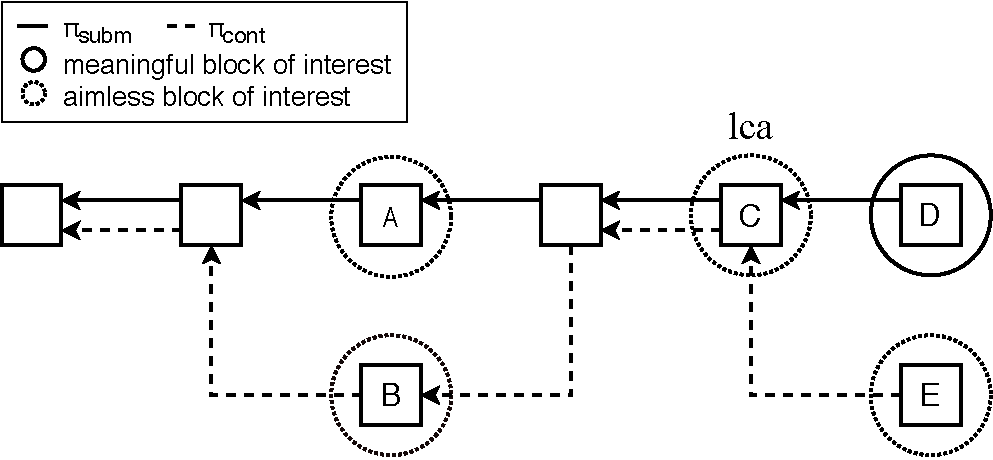
\includegraphics[width=0.6\columnwidth]{figures/boi-position.pdf}
    \end{center}
    \caption{Fork of two proofs.
    Solid lines connect blocks of $\pis$,
    and dashed lines connect blocks of $\pic$.
    In this configuration,
    blocks in dashed circles are aimless blocks of interest, and the block
    in the solid circle is a meaningful block of interest. Blocks B, C and E are
    aimless because they exist in $\pic$. Block A is aimless because it
    belongs to the subchain $\pis\{{:}\lca\}$
    }
    \label{fig:boi-position}
\end{figure}

\subsection{Subset of Proofs}

Now that we have achieved to freely retrieve $\pis$, we can start
sketching methodologies that benefit from this schema but another challenge we
had to face is that the protocol of NIPoPoWs dependents on DAG which is a
hashmap data structure

Our first realization was that instead of creating a DAG of $\pis$ and
$\pic$, we can rather require

\[ \pis\{:\textrm{LCA}\} \subseteq \pic\{:\textrm{LCA}\} \]
This way, we avoid the burden of maintaining auxiliary structures DAG and
ancestors on-chain. The implementation of \texttt{subset} is displayed in
listing~\ref{listing:subset}. The complexity of the function is \[
\mathcal{O}(|\pis\{:LCA\}| + |\pic\{:LCA\}]|) \]

\lstinputlisting[language=Solidity, label={listing:subset},
caption={Implementation of subset}]{code/Subset.sol}

\begin{figure}[ht]
\begin{subfigure}{.5\textwidth}
  \centering
  % include first image
  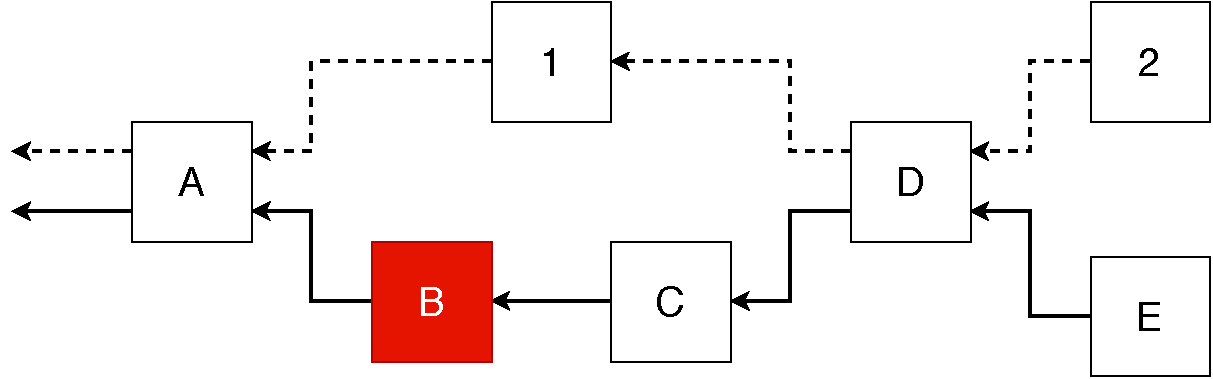
\includegraphics[width=6cm]{../images/Subset_1.pdf}
  \caption{Valid $\pi_{cont}$ before using subset}
  \label{figure:DAG_usage}
\end{subfigure}
\begin{subfigure}{.5\textwidth}
  \centering
  % include second image
  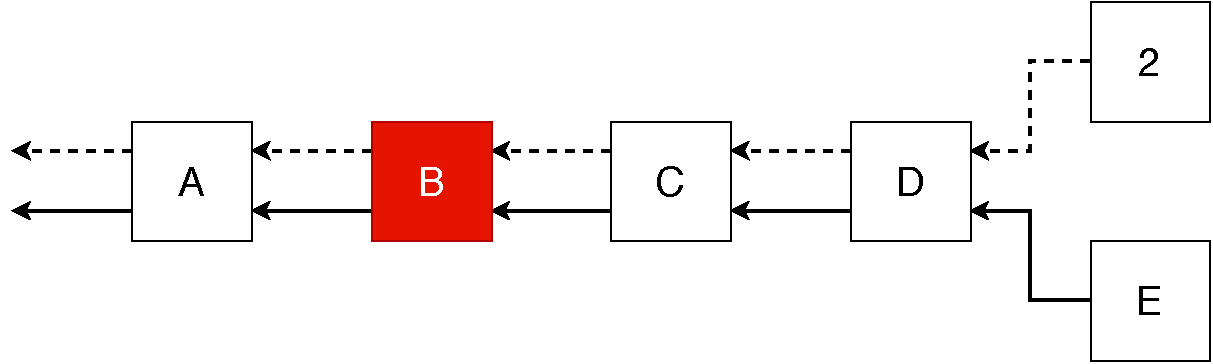
\includegraphics[width=6cm]{../images/Subset_2.pdf}
  \caption{Valid $\pi_{cont}$ after using subset}
  \label{figure:DAG_usage}
\end{subfigure}
\caption{Blocks connected with solid lines indicate $\pi_{exist}$ and blocks
connected with dashed lines indicate $\pi_{cont}$}
\label{fig:fig}
\end{figure}


The gas consumption difference between $subset$ and $DAG+ancestors$ is
displayed at figure~\ref{figure:DAG_vs_subset}. $Subset$ solution is
approximately 2.7 times more efficient.

\begin{figure}
\centering
\begin{tikzpicture}
    \begin{axis}[
        y tick label style={/pgf/number format/.cd,%
          set thousands separator={,},
          fixed},
        legend pos=north west,
        scaled y ticks = false,
        grid=major,
        xlabel={Proof size},
        ylabel={Gas consumption x 1.000}]
    \addplot table [col sep=comma] {data/DAG_ancestors.csv};
    \addplot table [col sep=comma] {data/subset.csv};
    \legend{$DAG+ancestors$,$Subset$};
\end{axis}
\end{tikzpicture}
\caption{Gas consumption for DAG+ancestors and subset}
\label{figure:DAG_vs_subset}
\end{figure}


\subsubsection{Subset complexity and limitations}

Requiring $\pis$ to be a subset of $\pic$ greatly reduces gas, but
the complexity of the $subset$ algorithm is high since both proofs have to be
iterated from $Gen$ until $lca_e$ and $lca_c$, respectively. Generally, we
expect from an adversary to provide a proof of a chain that is a fork of the
honest chain at some point relatively close to the tip. This is due to the fact
that the ability of an adversary to sustain a fork chain exponentially weakens
as the honest chain progresses. This means that the length of $\pi$, $|\pi|$ is
expected to be considerably close to $|\pi\{{:}lca\}|$, and thus the complexity of
\texttt{subset()} effectively becomes $\mathcal{O}(2|\pi|)$.

In realistic cases, where LCA lies around index 250 of the proof, the gas cost
of \texttt{subset()} is approximately $20{,}000{,}000$ gas units, which makes it
inapplicable for real chains since it exceeds the block gas limit of the
Ethereum blockchain by far.

\subsection{Minimal Fork} By combining the above observations, we
derive that $\pic$ can be truncated into $\pic\{\lca{:}\}$ without affecting
the correctness of the protocol. We term this truncated proof $\pitr$.
Security is preserved by requiring $\pitr$ to be a \emph{minimal fork} of
$\pis$. A minimal fork is a fork chain that shares exactly one common block
with the main chain. A proof $\tilde\pi$, which is minimal fork of $\pi$, has
the following attributes:

\begin{enumerate}
    \item $\pi_1[lca] = \pi_2[0]$
    \item $\pi_1[lca{:}] \cap \pi_2[1{:}] = \emptyset$
\end{enumerate}

By requiring $\pitr$ to be a minimal fork of $\pis$, we prevent adversaries
from dispatching an augmented $\pitr$ to claim better score against $\pis$.
Such an attempt is displayed in Figure~\ref{fig:adversary-minimal-fork}.

\begin{figure}[h]
    \begin{center}
        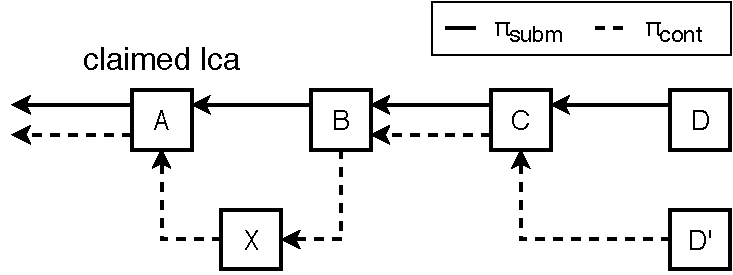
\includegraphics[width=0.5\columnwidth]{figures/adversary-minimal-fork.pdf}
    \end{center}
    \caption{An adversary attests to contest with a malformed proof. Adversary
        proof consists of blocks \{A, X, B, C, D'\} that achieve better score
        against submit proof \{A, B, C, D\}. This attempt is rejected due to
        the minimal-fork requirement.}
    \label{fig:adversary-minimal-fork}
\end{figure}

The implementation of minimal-fork is shown in listing~\ref{listing:disjoint}.
The complexity of \texttt{minimalFork()} is: \[ \mathcal{O}(|\pis\{\lca{:\}}|
\times |\pitr|) \]

\lstinputlisting[language=Solidity, label={listing:disjoint},
caption={Implementation for minimal fork}]{code/Disjoint.sol}

In Algorithm~\ref{alg:minimal-fork}, we show how the minimal fork technique is
incorporated into our client replacing DAG and ancestors. In
Figure~\ref{fig:minimal-fork} we show how the performance of the client
improves. We use the same test case as in \emph{hash-and-resubmit}.

\renewcommand{\genesis}{\textsf{G}}

\begin{algorithm}

    \label{alg:minimal-fork}
    \caption{The \textsf{NIPoPoW} client using the minimal fork technique}

    \begin{algorithmic}[1]

    \Contract{crosschain}
    \State $\textsf{events} \gets \bot;$ $\genesis \gets \bot$
    \Function{\sf initialize}{$\genesis_{remote}$}
        \State \genesis $\gets \genesis_{remote}$
    \EndFunction
    \Function{\sf submit}{$\pis$, $e$}
        \State \textsf{require}($\pis$[0] = $\genesis$)
        \State \textsf{require}($\textsf{events$[e]$} = \bot$)
        \State \textsf{require}($\textsf{valid-interlink}(\pis)$)
        \State \textsf{events$[e]$.hash} $\gets$ \textsf{H}($\pis$)
        \State \textsf{events$[e]$.pred} $\gets$
        \textsf{evaluate-predicate}(\textsf{$\pis$}, $e$)
    \EndFunction
    \Function{\sf contest}{$\pisa$, $\pitr$, $e$, $f$}
        \Comment{$f$: fork index}
        \State \textsf{require}($\pitr$[0] = $\pisa[f]$)
        \Comment{check fork head}
        \State \textsf{require}(\textsf{events}$[e]$ $\ne$ $\bot$)
        \State \textsf{require}(\textsf{events$[e]$.hash} $=$ \textsf{H}($\pisa$))
        \State \textsf{require}(\textsf{valid-interlink}($\pitr$))
        \State \textsf{require}(\textsf{minimal-fork}($\pisa$,
        $\pitr$, $f$))
        \State \textsf{require}(\textsf{score}($\pitr$)
            $>$ \textsf{score}($\pisa[f:]$))
        \State \textsf{events$[e]$.pred} $\gets$
            \textsf{evaluate-predicate}($\pitr$, $e$)
    \EndFunction
    \Function{\sf minimal-fork}{$\pi_1$, $\pi_2$, $f$}
        \For{$p\ in\ \pi_1$}
            \If{$p \in \pi_2$}
                \State\Return false
            \EndIf
        \EndFor
    \EndFunction
    \EndContract
    \vskip8pt
    \end{algorithmic}
\end{algorithm}



By applying the minimal-fork technique, he achieve a 55\% decrease in gas
consumption. \emph{Submit} phase now costs {4{,}700{,}000} gas, and
the \emph{contest} phase costs {4{,}900{,}000} million gas. This is a notable
result, since each phase now fits inside an Ethereum block.

\begin{figure}[H]
    \begin{center}
        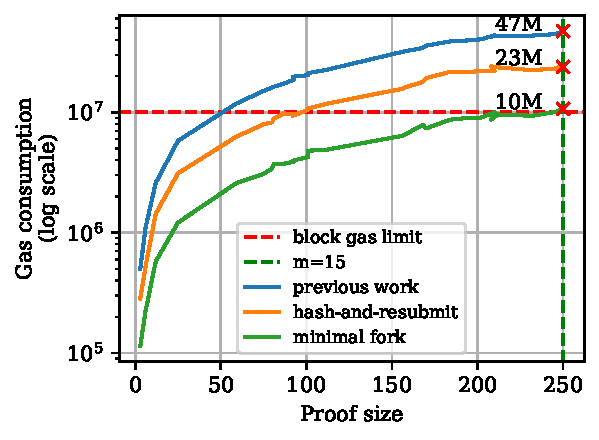
\includegraphics[width=0.6\columnwidth]{figures/minimal-fork.pdf}
    \end{center}
    \caption{Performance improvement using minimal fork (lower is better). The
        gas consumption is decreased by approximately 55\%.}
    \label{fig:minimal-fork}
\end{figure}

\section{Processing Fewer Blocks}

The complexity of most demanding on-chain operations of the verifier are linear
to the size of the proof. This includes the proof validation and the evaluation
of score. We now present two techniques that allow for equivalent operations of
constant complexity.

\subsection{Optimistic Schemes} In smart contracts, in order to ensure that users
comply with the underlying application's rules, certain actions need to be
performed on-chain, e.g. verification of data, balance checks, etc. In a
different approach, actions that deviate from the protocol are reverted after
honest users indicate them, not allowing diverging entities to gain advantages.
Such applications that do not check the validity of actions by default, but
rather depend on the intervention of honest users are characterized
``optimistic''. In the Ethereum community, several projects ~\cite{piza,
plasma, rollups-1, rollups-2} have emerged that incorporate the notion of
optimistic interactions. We observe that such a schema can be embedded into the
NIPoPoW protocol, resulting in significant performance gain.

We discussed how the verification in the NIPoPoW protocol is realized in two
phases. In \emph{submit} phase, the verification of the $\pis$ is performed.
This is necessary in order to prevent adversaries from injecting blocks that do
not belong to the chain, or changing existing blocks. A proof is valid for
submission if it is \emph{structurally correct}. Correctly structured NIPoPoWs
have the following requirements: (a) the first block of the proof is the
genesis block of the underlying blockchain and (b) every block has a valid
interlink.

Asserting the existence of genesis in the first index of a proof is an
inexpensive operation of constant complexity. However, confirming the interlink
correctness of all blocks is a process of linear complexity to the size of the
proof. Albeit the verification is performed in memory, sufficiently large
proofs result into costly submissions since their validation consist the most
demanding function of the \emph{submit} phase. In
Table~\ref{tab:valid-interlink-cost} we display the cost of
\textsf{valid-interlink} function which determines the structural correctness
of a proof in comparison with the overall gas used in \textsf{submit}.

\begin{table}[h]
\begin{tabular}{|c|c|c|}
\hline
\textbf{Process} & \textbf{Gas cost} & \multicolumn{1}{l|}{\textbf{Total \%}} \\ \hline
\textsf{verify-interlink} & 2,200,000         & 53\%                                     \\ \hline
\textsf{submit}           & 4,700,000         & 100\%                                    \\ \hline
\end{tabular}
\caption{Gas usage of \textsf{verify-interlink} compared to the overall
gas consumption of \textsf{submit}.}
\label{tab:valid-interlink-cost}
\vspace*{-5mm}
\end{table}


\newcommand{\dispute}{\emph{dispute\ }}

\subsection{Dispute Phase} We observe that the addition of a phase in
our protocol alleviates the burden of verifying all elements of the proof by
enabling the indication of an individual incorrect block. This phase, which we
term \dispute phase, leverages selective verification of the submitted proof at
a certain index. As a constant operation, this significantly reduces the gas
cost of the verification process.

In the NIPoPoW protocol, when a proof $\pis$ is submitted by $\es$, it is
retrieved by a node $\ec$ from the calldata and the proof is checked for its
validity \emph{off-chain}. We observe that, in
order to prove a structurally invalid $\pis$, $\ec$ only needs to
indicate the index in which $\pis$ fails the interlink verification. In the
protocol that incorporates \emph{dispute} phase, $\ec$ calls
$\textsf{dispute}$($\pisa$, $i$) for a structurally incorrect proof, where $i$
indicates the disputing index of $\pisa$. Therefore, only one block is
interpreted \emph{on-chain} rather than the entire span of $\pisa$.

Note that this additional phase does not imply increased rounds of
interactions between $\es$ and $\ec$. If $\pis$ is invalidated in
\emph{dispute} phase, then \emph{contest} phase is skipped. Similarly, if
$\pis$ is structurally correct, but represents a dishonest chain, then $\ec$
proceeds directly to \emph{contest} phase without the invocation of \emph{dispute}.

\begin{table}
\centering
\begin{tabular}{ccccccc|cc}
            & \textbf{Phase} & \textbf{Gas} &  &              & \textbf{Phase} & \textbf{Gas} & \textbf{Phase} & \textbf{Gas} \\ \cline{2-3} \cline{6-9}
 & submit  & 4.7 &  &  & submit  & 2.2 & submit  & 2.2 \\
 & contest & 4.9 &  &  & dispute & 1.3 & contest & 4.9 \\ \cline{2-3} \cline{6-9}
\textbf{I.} & \textbf{Total} & \textbf{9.6} &  & \textbf{II.} & \textbf{Total} & \textbf{3.5} & \textbf{Total} & \textbf{7.1}
\end{tabular}

\caption{Performance per phase. Gas units are displayed in millions.
\textbf{I}: Gas consumption prior to dispute phase incorporation. \textbf{II}:
Gas consumption for two independent sets of interactions submit/dispute and
submit/contest.}

\label{tab:dispute-cost}
\end{table}


In Table~\ref{tab:dispute-cost} we display the gas consumption for
two independent cycles of interactions:
\begin{enumerate}
    \item \emph{Submit} and \emph{dispute} for is structurally incorrect
        $\pis$.
    \item \emph{Submit} and \emph{contest} for structurally correct
        $\pis$ that represents a dishonest chain.
\end{enumerate}

\noindent In Algorithm~\ref{alg:dispute-best-level}, we show the implementation
of the \emph{dispute} phase. The integration of \emph{dispute} phase leaves
\textsf{contest} unchanged.

\subsection{Isolating the Best Level} As we discussed, \emph{dispute}
and \emph{contest} phases are mutually exclusive. Unfortunately, the same
constant-time verification as in the \emph{dispute} phase cannot be applied in a
contest without increasing the rounds of interactions for the users. However,
we derive a major optimization for the \emph{contest} phase by observing the
process of score evaluation.

In NIPoPoWs, after the last common ancestor is found, each proof fork
is evaluated in terms of proof-of-work score. Each level encapsulates a different
score of proof-of-work, and the level with the best score is representative
of the underlying proof. Since the common blocks of the two proofs naturally
gather the same score, only the disjoint portions need to be addressed.
Consequently, the position of the $\lca$ determines the span of the proofs that
will be included in the score evaluation process. Furthermore, it is impossible
to determine the score of a proof in the \emph{submit} phase because the position
of $\lca$ is yet unknown.

After $\pis$ is retrieved from the calldata, the score of both proofs is
calculated. This means that the level in which each proof encapsulates the
most proof-of-work for each proof is known to $\ec$. In the light of this
observation, $\ec$ only submits the blocks which consist the \emph{best level}
of $\pic$. The number of these blocks is constant, as it is determined by the
security parameter $m$, which is irrelevant to the size of the underlying
blockchain. We illustrate the blocks that participate in the formulation of a
proof's score and the best level of contesting proof in
Figure~\ref{fig:score-at-levels}.

\begin{figure}[!h]
    \begin{center}
    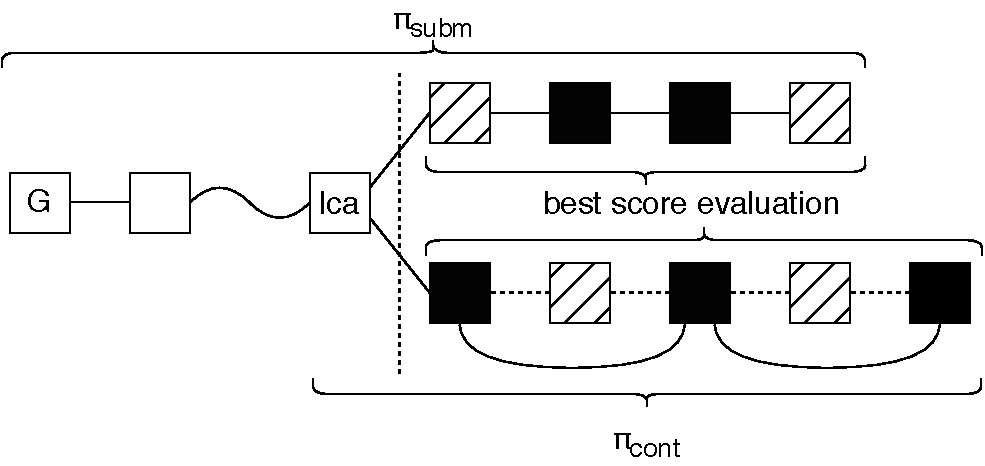
\includegraphics[width=0.6\columnwidth]{figures/blocks-of-best-level.pdf}
    \end{center}
    \caption{Fork of two proofs. Striped blocks determine the
    score of each proof. Black blocks belong to the level that
    has the best score. Only black blocks are part of the best level of the
    contesting proof.}
    \label{fig:score-at-levels}
\end{figure}


The calculation of the best level of $\pic$ is an \emph{off-chain} process.
An adversarial $\ec$ is certainly able to dispatch a level of $\pic$ which is
different than the best level. However, this is an irrational action, since
different levels only undermine the score of $\pic$. On the contrary, due to
the consistency property of \emph{hash-and-resubmit}, $\pis$ cannot be altered.
We denote the best level of $\pitr$ as $\pitrl$.

In Algorithm~\ref{alg:dispute-best-level}, we show the implementation of the
\emph{contest} phase under the best-level enhancement. The utilization of
this methodology greatly increases the performance of the client,
because the complexity of the majority of $\textsf{contest}$ functions is
related to the size of $\pic$. In Table~\ref{tab:best-level-cost}, we
demonstrate the difference in gas consumption in the \emph{contest} phase after
using \emph{best-level}. The performance of most functions is increased by
approximately 85\%. This is due to the fact that the size of $\pic$ is
decreased accordingly. For $m=15$, $\pitrl$ consists of 31 blocks, while
$\pitr$ consists of 200 blocks.  Notably, the calculation of score for $\pitrl$
needs 97\% less gas. We achieve such a discrepancy because the process of score
calculation for multiple levels demands the use of a temporary hashmap which is
a storage structure. In contrast, the evaluation of the score of an individual level
is performed entirely in memory.

\begin{table}[]
\begin{tabular}{|c|l|r|r|l|r|r|}
\cline{1-1} \cline{3-4} \cline{6-7}
\textbf{Process} &
   &
  \multicolumn{1}{c|}{\textbf{\begin{tabular}[c]{@{}c@{}}Gas\\ Cost\end{tabular}}} &
  \multicolumn{1}{c|}{\textbf{Total}} &
   &
  \multicolumn{1}{c|}{\textbf{\begin{tabular}[c]{@{}c@{}}Gas\\ Cost\end{tabular}}} &
  \multicolumn{1}{c|}{\textbf{Total}} \\ \cline{1-1} \cline{3-4} \cline{6-7}
  \textsf{valid-interlinks} &            & 900,000   & 18\%  &             & 120,000   & 10\%  \\ \cline{1-1} \cline{3-4} \cline{6-7}
  \textsf{minimal-fork}     &            & 1,900,000 & 39\%  &             & 275,000   & 18\%  \\ \cline{1-1} \cline{3-4} \cline{6-7}
  \textsf{score} (p1)       &            & 750,000   & 16\%  &             & 750,000   & 51\%  \\ \cline{1-1} \cline{3-4} \cline{6-7}
  \textsf{score} (p2)       &            & 950,000   & 19\%  &             & 20,000    & 1\%   \\ \cline{1-1} \cline{3-4} \cline{6-7}
other            &            & 400,000   & 8\%   &             & 300,000   & 20\%  \\ \cline{1-1} \cline{3-4} \cline{6-7}
\textsf{contest}          & \textbf{I} & 4,900,000 & 100\% & \textbf{II} & 1,465,000 & 100\% \\ \cline{1-1} \cline{3-4} \cline{6-7}
\end{tabular}
\caption{Gas usage in contest. I: before utilizing best level. II: after
utilizing best level.}
\label{tab:best-level-cost}
\end{table}


In Figure ~\ref{fig:dispute-best-level}, we illustrate the performance gain of
the client using \emph{dispute} phase and the best-level contesting proof. The
aggregated gas consumption of \emph{submit} and \emph{contest} phases is
reduced to 3,500,000 gas. This is a critical threshold regarding applicability of
the contract, since a cycle of interactions now effortlessly fits inside a
single Ethereum block.

\begin{algorithm}
    \caption{\label{alg:dispute-best-level}The \textsf{NIPoPoW} client enhanced
        with dispute phase and best-level contesting}

    \begin{algorithmic}[1]

    \Contract{crosschain}
    \State $\textsf{events} \gets \bot;$ $\genesis \gets \bot$
    \Function{\sf initialize}{$\genesis_{remote}$}
        \State $\genesis$ $\gets \genesis_{remote}$
    \EndFunction
    \Function{\sf submit}{$\pis$, $e$}
        \State \textsf{require}($\pis$[0] = $\genesis$)
        \State \textsf{require}($\textsf{events$[e]$} = \bot$)
        \State \textsf{events$[e]$.hash} $\gets$ \textsf{H}($\pis$)
        \State \textsf{events$[e]$.pred} $\gets$
        \textsf{evaluate-predicate}(\textsf{$\pis$}, $e$)
    \EndFunction
    \Function{\sf dispute}{$\pisa$, $e$, $i$}
        \Comment{$i$: dispute index}
        \State \textsf{require}(\textsf{events}$[e]$ $\ne$ $\bot$)
        \State \textsf{require}(\textsf{events$[e]$.hash} $=$ \textsf{H}($\pisa$))
        \State \textsf{require}($\neg \textsf{valid-single-interlink}(\pis, i)$)
        \State \textsf{events$[e]$} $\gets$ $\bot$
    \EndFunction
    \Function{\sf valid-single-interlink}{$\pi$, $i$}
        \State $l\gets\pi[i].\mathsf{level}$
        \If{$\pi[i{+}1].\mathsf{intelink}[l] = \pi[i]$}
        \State \Return true
        \EndIf
        \State \Return false
    \EndFunction
    \Function{\sf contest}{$\pisa$, $\pitrl$, $e$, $f$}
        \State \textsf{require}($\pitrl$[0] = $\pisa[f]$)
        \State \textsf{require}(\textsf{events}$[e]$ $\ne$ $\bot$)
        \State \textsf{require}(\textsf{events$[e]$.hash} $=$ \textsf{H}($\pisa$))
        \State \textsf{require}(\textsf{valid-interlinks}($\pitrl$))
        \State \textsf{require}(\textsf{minimal-fork}($\pisa$,
        $\pitrl$, $f$))
        \State \textsf{require}(\textsf{score-at-level}($\pitrl$)
        $>$ \textsf{score}($\pisa[f{:}]$))
        \State \textsf{events$[e]$.pred} $\gets$
            \textsf{evaluate-predicate}($\pitrl$, $e$)
    \EndFunction
    \Function{\sf score-at-level}{$\pi$}
        \State $l \gets \pi[-1].\textsf{level}$
        \Comment{pick proof level from a block}
        \State $score \gets 0$
        \Comment{set score counter to 0}
        \For{b in $\pi$}
            \State \textsf{require}(b.\textsf{level} = $l$)
            \State $score \gets score {+} 2^l$
        \EndFor
        \State \Return{score}
    \EndFunction
    \EndContract
    \vskip8pt
    \end{algorithmic}
\end{algorithm}



\begin{figure}[!h]
    \begin{center}
        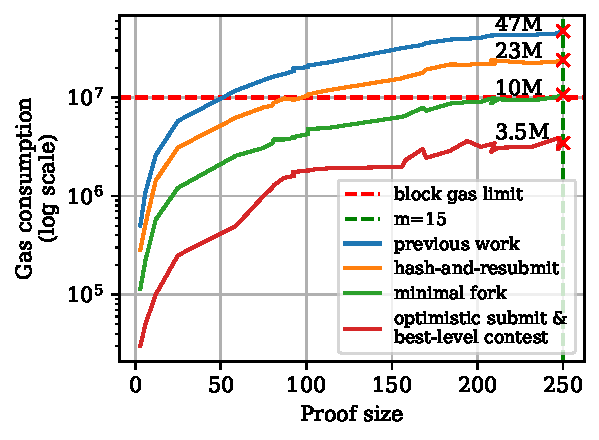
\includegraphics[width=0.6\columnwidth]{figures/dispute-best-level.pdf}
    \end{center}
    \caption{Performance improvement using optimistic schema in submit phase
        and best level proof in contesting proof (lower is better). Gas
        consumption is decreased by approximately 65\%.}
    \label{fig:dispute-best-level}
\end{figure}
\newpage

\section{Resilience Against DOS Attacks}

We will now examine whether an adversary can perform an attack to the verifier
by submitting a dishonest proof that cannot be contested due to gas exhaustion.
In this scenario, an adversary could submit a fraud proof that cannot be
invalidated by honest parties; this would be a significant security
vulnerability in the protocol.

As we already discussed, the gas consumption for contesting a proof that
represent dishonest chains that is relatively short fork of the honest chain
is around $1.3$ million gas. This cost, however, increases as the fork point of
the fraud proof is getting closer to genesis. This is due to the fact that
the operation of calculating the score of each proof is proportional to the
number of disjoint blocks. This means that the most expensive scenario of
contesting is when $\pis$ represents a dishonest chain that forks the honest
chain at genesis.

Our experiments show that the gas cost of contesting a proof for a dishonest
chain that spans almost the same number of blocks as the honest chain and forks
the honest chain in genesis is around $5.9$ million gas. This illustrates that
the verifier is resilient to Denial-of-Service attack even in the most extreme
scenarios. In the following Section, we also provide a cryptoeconomic analysis
about the collateral needed in order to provide incentives to honest proves
that need to contest genesis forks.

